\chapter{Signal Modeling}

How do we produce a signal hypothesis that we can test?
Mostly just a bunch of software.

\section{Monte-Carlo Simulation}

    Need to cover MadGraph, Pythia, and Geant4.

\section{Signal Combination}

    The cross-section and kinematic distributions of the di-Higgs production processes depend fundamentally on a number of coupling constants between the Higgs and other particles.
    Of particular interest in this analysis are \kl for the Higg's self-coupling and \kvv for the \HHVV coupling.
    The values of \kl and \kvv have loose experimental constraints \cite{EXOT-2016-31} \cite{HDBS-2018-18-witherratum} \cite{ATLAS-CONF-2019-049}, requiring analysis across a wide range of these coupling values.
    Unfortunately, MC generation is computationally expensive and time consuming.
    As such, only a handful of MC simulation samples for only a handful of coupling values are actually produced, and a sample combination technique is employed to model the signal hypothesis across the coupling parameter space.

    The process of combining a few samples in such a way as to model the entire parameter space of coupling constants is based on exploiting the underlying mathematics of the differential cross-section formula.
    By expanding the squared term of the sum of all Feynman diagram contributions, the cross-section can be expressed as a function of its coupling values \cite{ATLAS-CONF-2019-049}.
    In the case of VBF the differential cross-section depends on the three diagrams of Figure \ref{fig:tree_level_vbfhh} as:

    %\begin{equation} \label{eqn:ggf_hh_feynSum}
    %\frac{d\sigma(\kl, \kt)}{d \mhh}  = | A(\kt, \kl) |^2 = | \kl \kt M_{\bigtriangleup}(\mhh) + \kt^2 M_{\Box}(\mhh) |^2
    %\end{equation}

    %\begin{equation} \label{eqn:ggf_hh_feynExpand}
    %    = \kl^2 \kt^2 |M_{\bigtriangleup}(\mhh)|^2 +
    %    \kl \kt^3 [ M_{\bigtriangleup}^*(\mhh) M_{\Box}(\mhh) + M_{\Box}^*(\mhh) M_{\bigtriangleup}(\mhh) ] +
    %    \kt^4 |M_{\Box}|^2
    %\end{equation}

    %\begin{equation} \label{eqn:ggf_hh_feynSimple}
    %    = \kl^2 \kt^2 a_1(\mhh) + \kl \kt^3 a_2(\mhh) + \kt^4 a_3(\mhh)
    %\end{equation}


    The $a_i$ matrix element expansion values have a dependence on \mhh, which is not trivially derivable as an analytic function.
    Instead, for a given \kl, its cross-section in each \mhh bin can be mathematically determined by solving a set of linear equations for $a_1$, $a_2$, and $a_3$,
        using three different cross-section values (in the same \mhh bin) for three different \kl values.
    In practice, the cross-section values of these three \textit{basis} samples are represented by the yields from MC simulation, binned by their true \mhh.
    Once the $a_i$ values are obtained, event weights for every \kl values can be derived for one of the simulated samples (e.g.\ the SM sample),
        by taking the ratio between the true \mhh distributions of the target coupling and the SM.
    By applying these weights to the SM sample, one obtains a reweighted sample for the targeted \kl value.

    In order to obtain a reweighted distribution at reconstruction-level, the truth \mhh value is stored in the SM sample, and the weights are applied to the events remaining after reconstruction and selection.
    In this approach, an assumption is made that the acceptance varies approximately as a function of only \mhh.
    This assumption is validated on a fourth sample by comparing the distributions from the reweighted sample and a MC sample generated at some other point in \kl.

    The VBF HH process is modelled in a similar manner to the ggF process, but with some key differences.
    Most notably, the sample combination for VBF is not done at truth level.
    The kinematics of the VBF process involve both the Higgs pair and the VBF initial scatter jets.
    As such, the acceptance cannot be adequately described by only one variable (e.g.\ \mhh), rendering the truth re-weighting approach untenable.
    Instead, all of the basis VBF MC samples are run through reconstruction and selection.
    The signal distribution modelling is then performed by directly combining the reconstructed \mhh distributions of post-selection signal samples.

    The VBF to HH process involves 3 diagrams (Figure \ref{fig:tree_level_vbfhh}). 
    The squared-sum matrix element expansion then produces six terms, which are a function of three couplings (\kvv, \kl, \kv).
    The full modelling equation for VBF thus requires the combination of six different samples (see this section after I copy in the appendix).
    This particular combination of samples was chosen first, based on the samples available and, second, by an optimization procedure described in right here TODO.

    \begin{equation}
    \label{eqn:vbf_hh_6term_chosen}
    \begin{split}
        \frac{d\sigma}{d\mhh}(\kvv, \kl, \kv) =
            \left(\frac{68 \kappa_{2V}^{2}}{135} - 4 \kappa_{2V} \kappa_{V}^{2} + \frac{20 \kappa_{2V} \kappa_{V} \kappa_{\lambda}}{27} + \frac{772 \kappa_{V}^{4}}{135} - \frac{56 \kappa_{V}^{3} \kappa_{\lambda}}{27} + \frac{\kappa_{V}^{2} \kappa_{\lambda}^{2}}{9}\right) \times \frac{d\sigma}{d\mhh}{\left(1,1,1 \right)} \\
            + \left(- \frac{4 \kappa_{2V}^{2}}{5} + 4 \kappa_{2V} \kappa_{V}^{2} - \frac{16 \kappa_{V}^{4}}{5}\right) \times \frac{d\sigma}{d\mhh}{\left(\frac{3}{2},1,1 \right)} \\
            + \left(\frac{11 \kappa_{2V}^{2}}{60} + \frac{\kappa_{2V} \kappa_{V}^{2}}{3} - \frac{19 \kappa_{2V} \kappa_{V} \kappa_{\lambda}}{24} - \frac{53 \kappa_{V}^{4}}{30} + \frac{13 \kappa_{V}^{3} \kappa_{\lambda}}{6} - \frac{\kappa_{V}^{2} \kappa_{\lambda}^{2}}{8}\right) \times \frac{d\sigma}{d\mhh}{\left(1,2,1 \right)} \\
            + \left(- \frac{11 \kappa_{2V}^{2}}{540} + \frac{11 \kappa_{2V} \kappa_{V} \kappa_{\lambda}}{216} + \frac{13 \kappa_{V}^{4}}{270} - \frac{5 \kappa_{V}^{3} \kappa_{\lambda}}{54} + \frac{\kappa_{V}^{2} \kappa_{\lambda}^{2}}{72}\right) \times \frac{d\sigma}{d\mhh}{\left(1,10,1 \right)}  \\
            + \left(\frac{88 \kappa_{2V}^{2}}{45} - \frac{16 \kappa_{2V} \kappa_{V}^{2}}{3} + \frac{4 \kappa_{2V} \kappa_{V} \kappa_{\lambda}}{9} + \frac{152 \kappa_{V}^{4}}{45} - \frac{4 \kappa_{V}^{3} \kappa_{\lambda}}{9}\right) \times \frac{d\sigma}{d\mhh}{\left(1,1,\frac{1}{2} \right)} \\
            + \left(\frac{8 \kappa_{2V}^{2}}{45} - \frac{4 \kappa_{2V} \kappa_{V} \kappa_{\lambda}}{9} - \frac{8 \kappa_{V}^{4}}{45} + \frac{4 \kappa_{V}^{3} \kappa_{\lambda}}{9}\right) \times \frac{d\sigma}{d\mhh}{\left(1,-5,\frac{1}{2} \right)}
    \end{split}
    \end{equation}

    Discussion here will focus on the individual one-dimensional \kvv and \kl scans.
    Note that although \ref{eqn:vbf_hh_6term_chosen} involves six samples, the equation simplifies down to only three terms (and thus needs only three samples to combine) when \kvv and \kv are set to the Standard Model value of 1.
    In theory the same can be done to produce a 1D equation for \kvv (by setting \kl and \kv to 1), though this particular basis does not permit such a simplification.
    For \kl, the simplified three-term equation takes the form

    \begin{equation}
    \label{eqn:vbf_hh_3term_kl}
    \begin{split}
        \frac{d\sigma}{d\mhh}(\kvv=1, \kl, \kv=1) =
        \left(\frac{\kappa_{\lambda}^{2}}{9} - \frac{4 \kappa_{\lambda}}{3} + \frac{20}{9}\right) \times
            \frac{d\sigma}{d\mhh}{\left(1,1,1 \right)} \\
        \left(- \frac{\kappa_{\lambda}^{2}}{8} + \frac{11 \kappa_{\lambda}}{8} - \frac{5}{4}\right) \times
            \frac{d\sigma}{d\mhh}{\left(1,2,1 \right)} \\
        \left(\frac{\kappa_{\lambda}^{2}}{72} - \frac{\kappa_{\lambda}}{24} + \frac{1}{36}\right) \times
            \frac{d\sigma}{d\mhh}{\left(1,10,1 \right)}
    \end{split}
    \end{equation}



    This procedure has been successfully validated in its ability to accurately model a large range of coupling values (see \ref{fig:vbf_hh_validation}) and shown to produce reasonable distributions well beyond the Standard Model coupling values (\ref{fig:vbf_hh_preview}).

    \begin{figure}
    	\centering
        \subfloat[Validation against MC with $\kl=0$]{
            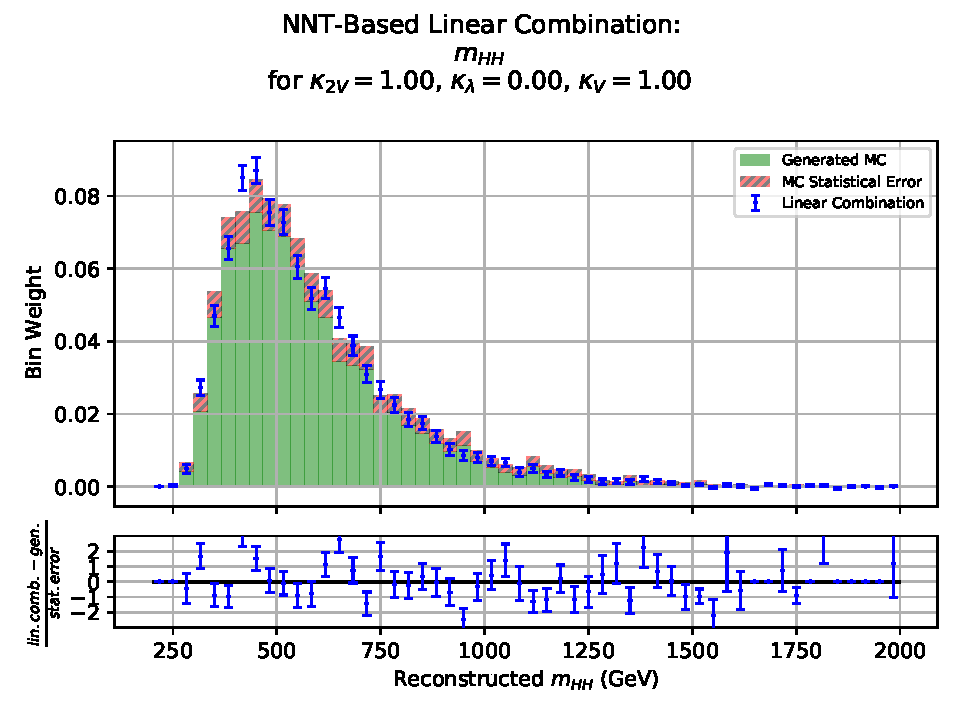
\includegraphics[width=0.32\linewidth,height=\textheight,keepaspectratio]{signal/reco_mHH_cvv1p00cl0p00cv1p00}
        }
        \subfloat[Validation against MC with $\kvv=0$]{
            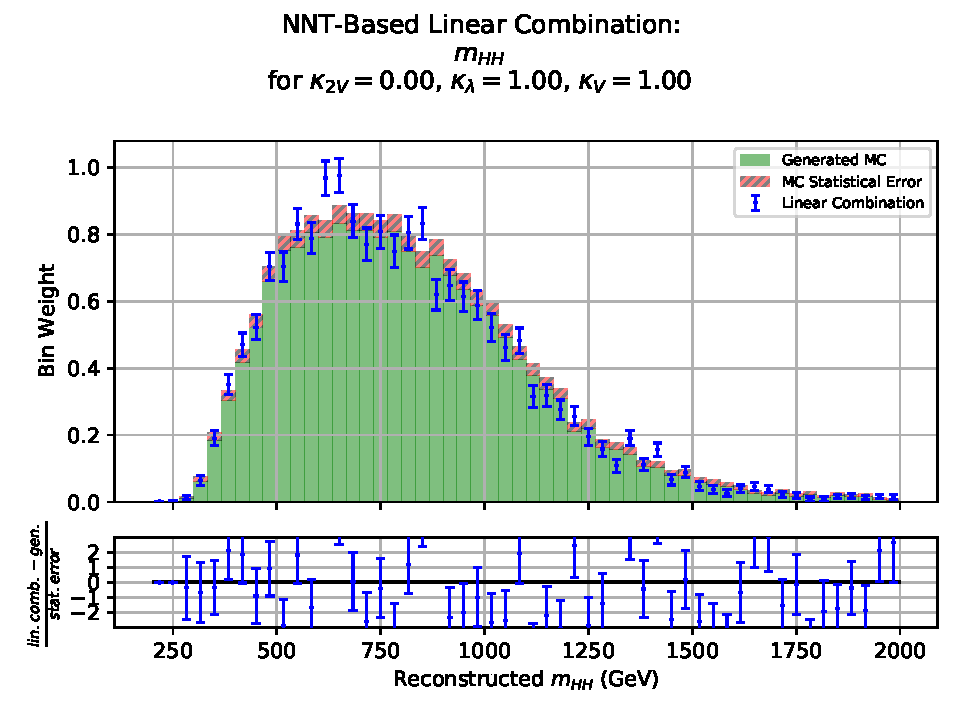
\includegraphics[width=0.32\linewidth,height=\textheight,keepaspectratio]{signal/reco_mHH_cvv0p00cl1p00cv1p00}
        }
        \subfloat[Validation against MC with $\kvv=3$]{
            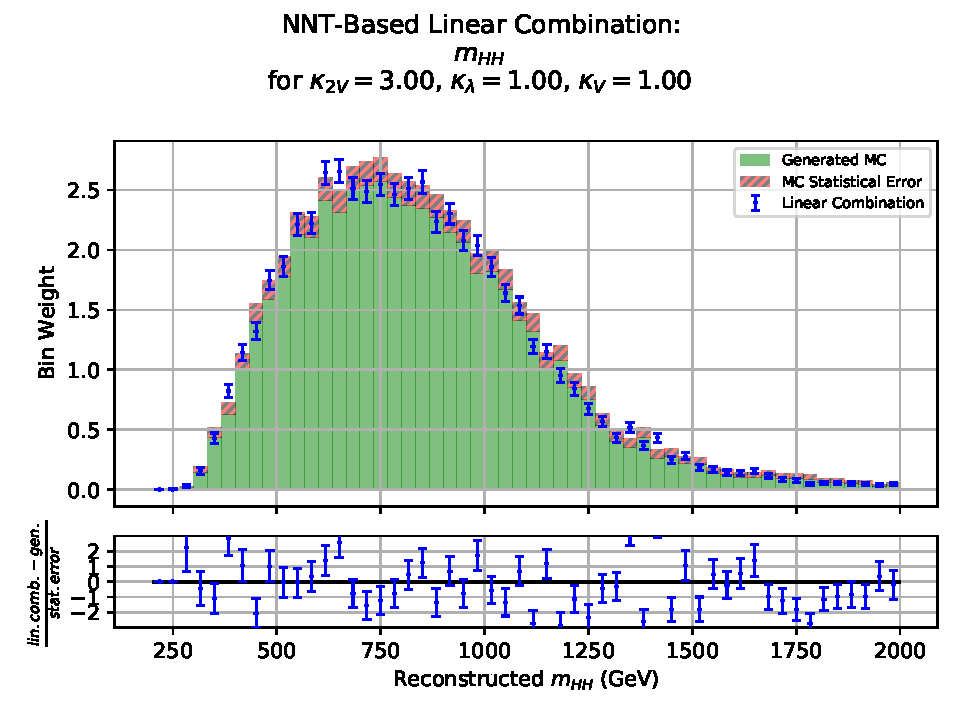
\includegraphics[width=0.32\linewidth,height=\textheight,keepaspectratio]{signal/reco_mHH_cvv3p00cl1p00cv1p00}
        }
        \caption{
            The six-term linear combination of samples is combined for various coupling values.
            The combined distribution shape (in blue) is compared against a Monte-Carlo sample (in green) which was generated for the same coupling values.
            The combination approach shows good agreement with the generated sample, indicating accurate modelling of the signal shape.
        }
        \label{fig:vbf_hh_validation}
    \end{figure}



    \begin{figure}
    	\centering
        \subfloat[Combination at  \kvv = -2]{
            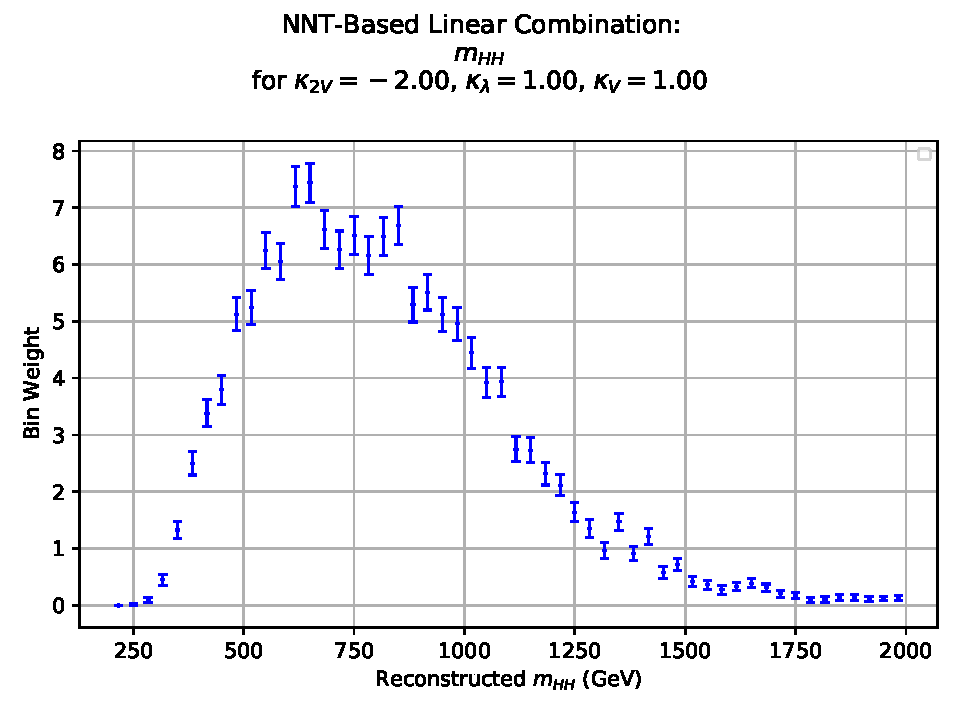
\includegraphics[width=0.44\linewidth,height=\textheight,keepaspectratio]{signal/preview_reco_mHH_new_cvv-2p00cl1p00cv1p00}
        }
        \subfloat[Combination at  \kl = -9]{
            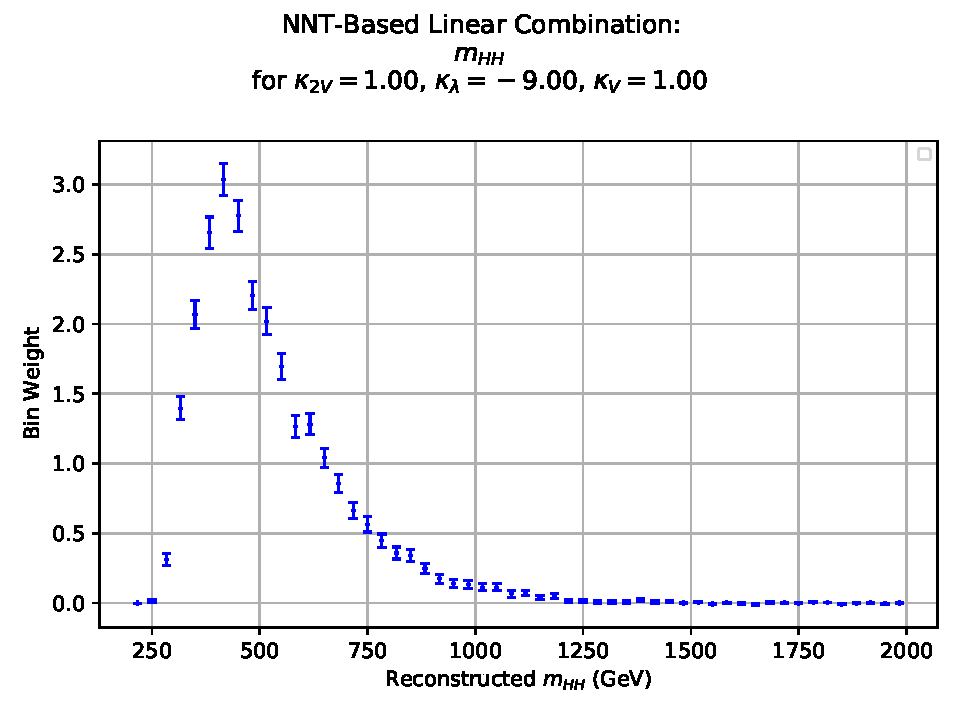
\includegraphics[width=0.44\linewidth,height=\textheight,keepaspectratio]{signal/preview_reco_mHH_new_cvv1p00cl-9p00cv1p00}
        }
        \caption{
            The six-term linear combination of samples is combined for coupling values very far from the Standard Model.
            There are no MC simulated samples to compare these points too, but the combined distributions at these points are smooth and well-behaved,
                indicating reasonable modelling of the distribution even at distant couplings.
        }
        \label{fig:vbf_hh_preview}
    \end{figure}


\section{VBF Full 3D Combination} \label{app:vbf3dcombination}

    The full cross section for the VBF to HH process involves three diagrams,

    \begin{equation}
    \label{eqn:vbf_hh_6term_amp}
    \sigma(\kvv, \kl, \kv) = |A|^2 = | \kv \kl M_s + \kv^2 M_t + \kvv M_x |^2
    \end{equation}

    Expanding the absolute square of the amplitude $A$ then yields six terms:

    \begin{equation}
    \label{eqn:vbf_hh_6term_generic}
    \sigma = \kv^2 \kl^2 a_1 + \kv^4 a_2 + \kvv^2 a_3 + \kv^3 \kl a_4 + \kv \kl \kvv a_5 + \kv^2 \kvv a_6
    \end{equation}

    As discussed earlier, this requires the combination of six different Monte-Carlo samples in order to model the signal hypothesis at any arbitrary point in \kvv, \kl, \kv space.
    In theory, with infinite events, the only requirement for these samples is that they are linearly independent of each other.
    In practice, the final samples are statistically limited, and different combinations of variations yield different statistical power.
    The 6-sample combination used in this analysis (\ref{tab:vbf_hh_6term_varlist} and \ref{eqn:vbf_hh_6term_chosen}) has been chosen specifically for its ability to avoid mismodelling errors.
    The method used to determine the overall performance of a basis is to check the number of negative bins generated
        in the \mhh distribution across all points in the two-dimensional \kvv,\kl space, as seen in \ref{fig:vbf_hh_6term_nWeight_grid}.
    As negative bin weights are unphysical, they indicate poor signal modelling.
    Thus, identifying a basis which minimizes the presence of negative weights ensures stable modeling of the signal hypothesis at all points in the coupling space (\ref{fig:vbf_hh_6term_validation} and \ref{fig:vbf_hh_6term_preview}).

    \begin{table}[] \centering
    \caption{6-Term VBF Combination Sample Variations}
    \label{tab:vbf_hh_6term_varlist}
    \begin{tabular}{ |l|l|l| }
        \hline
        \textbf {$\kappa_{2V}$} & \textbf {$\kappa_\lambda$} & \textbf {$\kappa_V$} \\
        \hline
            1   &   1 & 1   \\
            1.5 &   1 & 1   \\
            1   &   2 & 1   \\
            1   &  10 & 1   \\
            1   &   1 & 0.5 \\
            0   &  -5 & 0.5 \\
        \hline
    \end{tabular} \end{table}

    \begin{figure}
        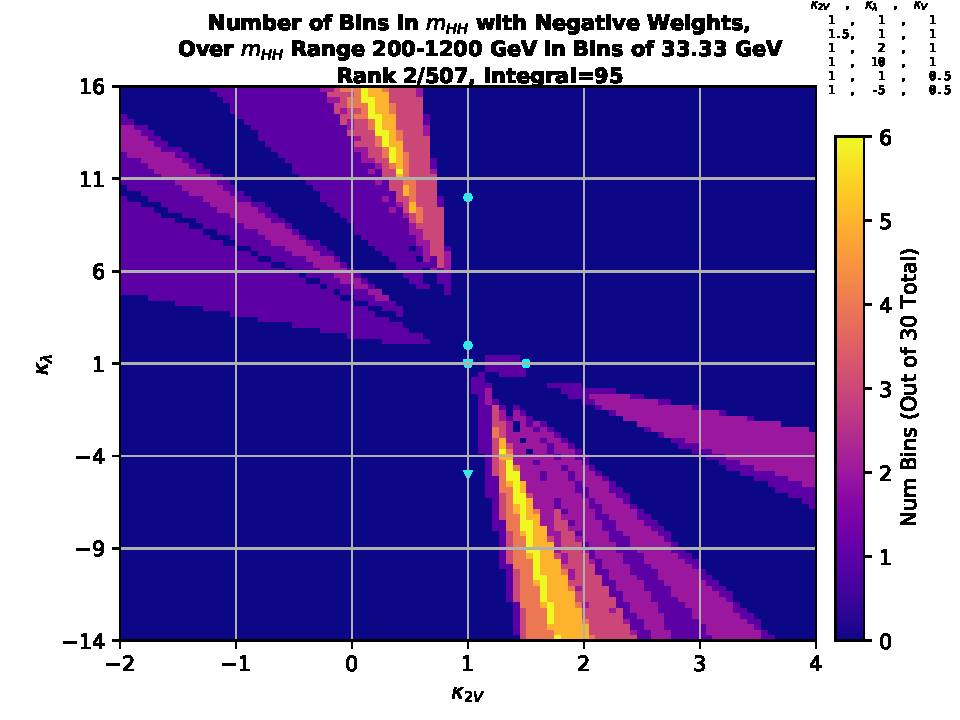
\includegraphics[width=\linewidth,height=\textheight,keepaspectratio]{signal/negative_weights_base}
        \caption{
            Frequency of negative bin weights in \mhh distribution across \kvv,\kl range.
            Brighter regions indicate more negative-weighted bins, and suggest less stable signal modelling.
            This particular combination of samples was chosen for how much of the space is ``dark",
                with darker regions indicating generally stable signal modelling.
            The table of coupling values in the upper right corner indicates the 6 MC samples
                (highlighted on the plot with cyan dots) used in the combination.
        }
        \label{fig:vbf_hh_6term_nWeight_grid}
    \end{figure}


    \begin{figure}
        \subfloat[Validation \kv = 1.5]{
            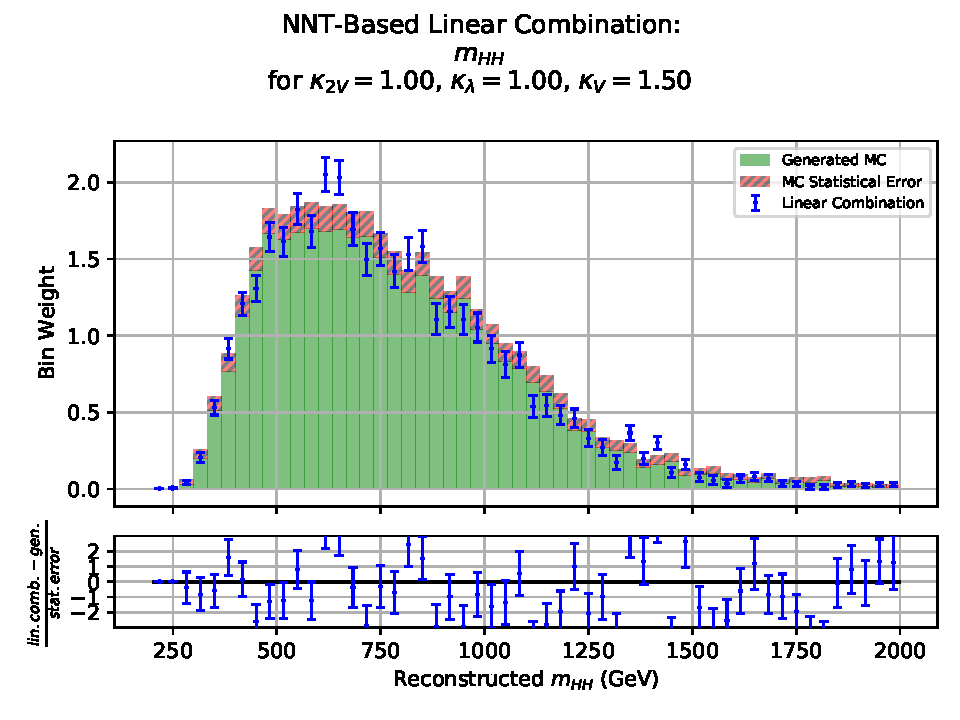
\includegraphics[width=0.5\linewidth,height=\textheight,keepaspectratio]{signal/reco_mHH_cvv1p00cl1p00cv1p50}
        }
        \subfloat[Validation \kl = 0]{
            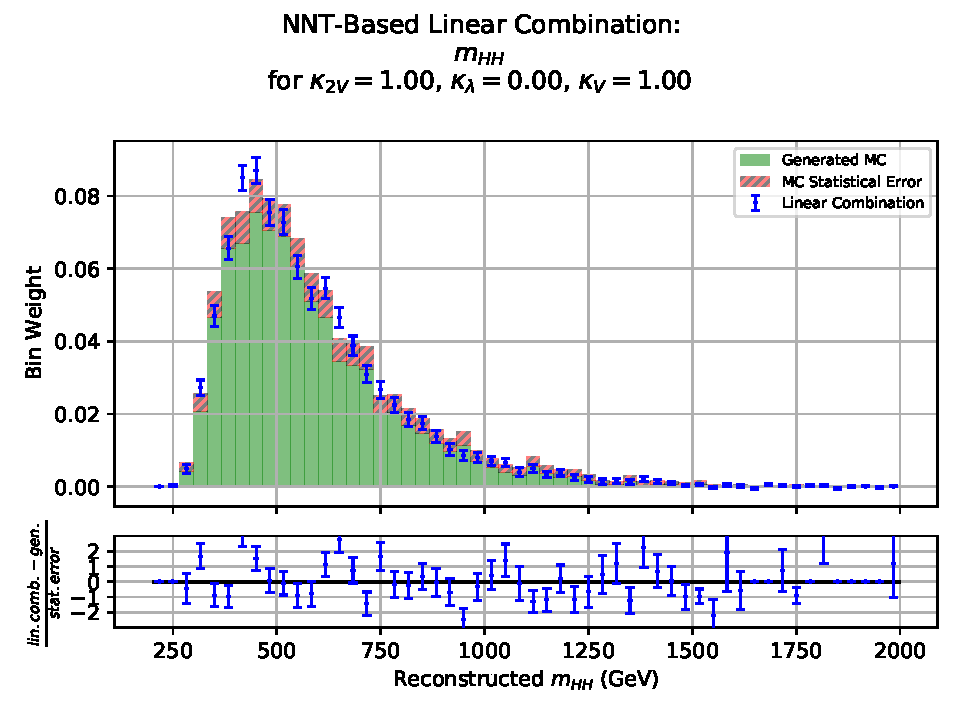
\includegraphics[width=0.5\linewidth,height=\textheight,keepaspectratio]{signal/reco_mHH_cvv1p00cl0p00cv1p00}
        }
        \caption{
            Validation of 6-term combination against MC generated at \kv = 1.5 and \kl = 0.
            The combination shows good agreement to the generated MC distributions.
        }
        \label{fig:vbf_hh_6term_validation}
    \end{figure}



    \begin{figure}
        \subfloat[Combined \mhh distribution at \kvv = 2.5, \kl = -10]{
            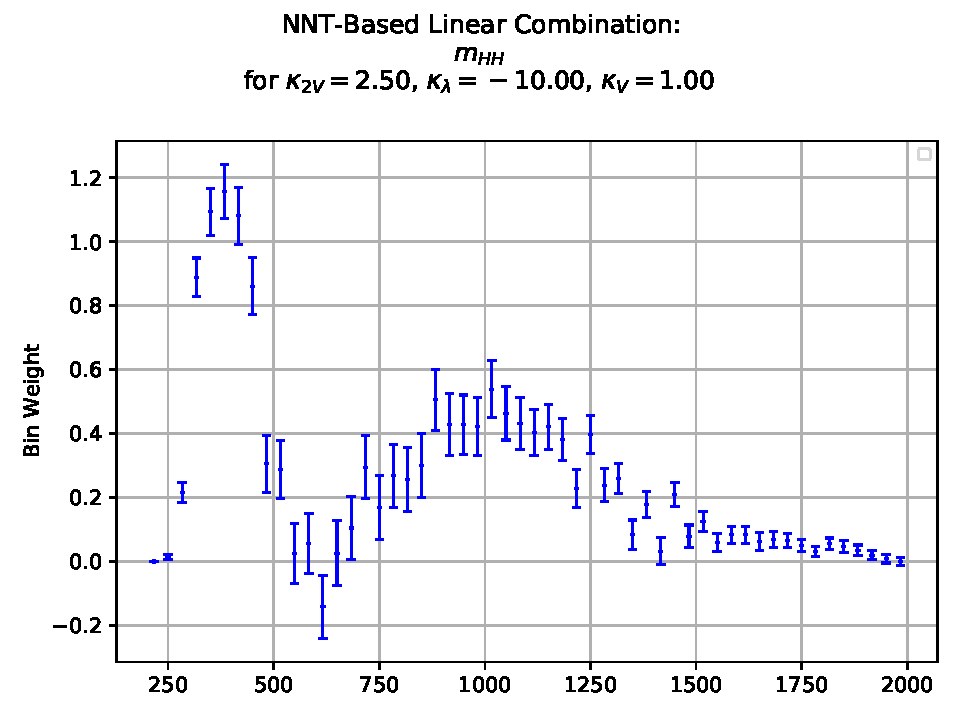
\includegraphics[width=0.5\linewidth,height=\textheight,keepaspectratio]{signal/preview_reco_mHH_new_cvv2p50cl-10p00cv1p00}
        }
        \subfloat[Combined \mhh distribution at \kvv = 2.0, \kl = -10]{
            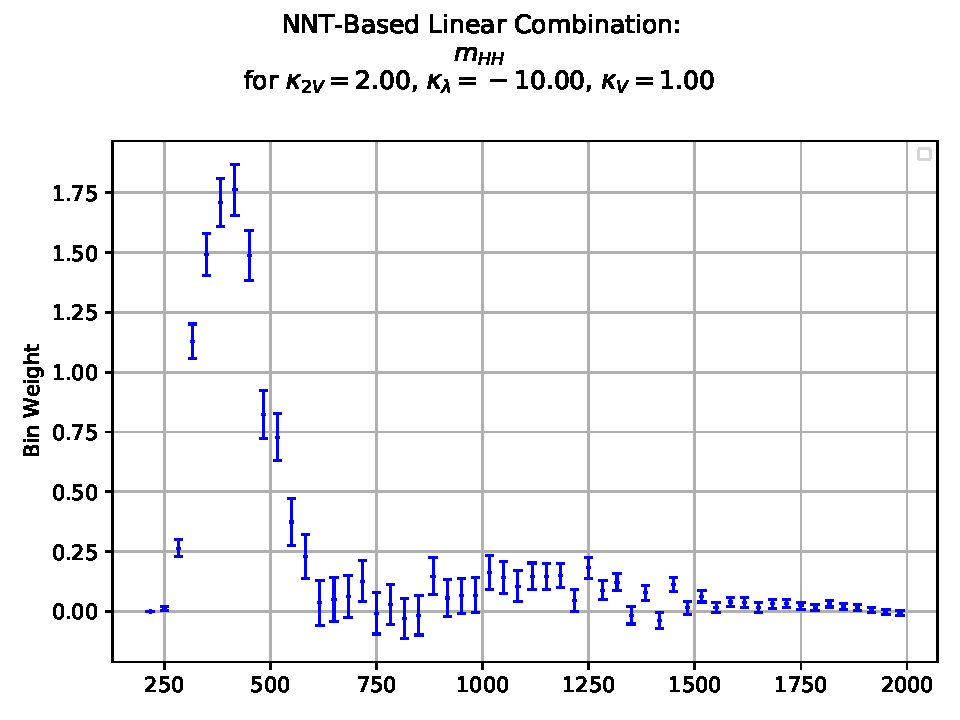
\includegraphics[width=0.5\linewidth,height=\textheight,keepaspectratio]{signal/preview_reco_mHH_new_cvv2p00cl-10p00cv1p00}
        }\\
        \subfloat[Combined \mhh distribution at \kvv = 0, \kl = 13]{
            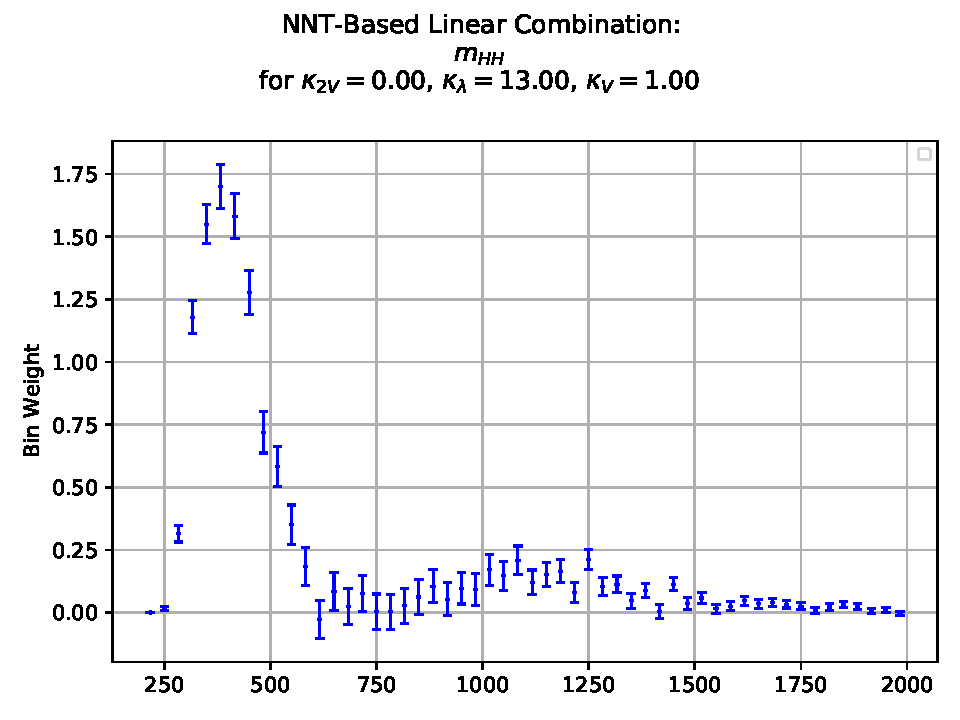
\includegraphics[width=0.5\linewidth,height=\textheight,keepaspectratio]{signal/preview_reco_mHH_new_cvv0p00cl13p00cv1p00}
        }
        \caption{
            \mhh distribution produced by the 6-term combination at points far from the SM.
            The combination produces smooth, well-behaved distributions at these points,
                suggesting the signal is well-modelled in these regions.
        }
        \label{fig:vbf_hh_6term_preview}
    \end{figure}



\section{Solidarity}
    
    Should this go here?
